
\documentclass[10pt]{article}
\usepackage[english]{babel}
\usepackage[utf8x]{inputenc}
\usepackage{graphicx}
\usepackage{minted}
\usemintedstyle{pastie}
\usepackage{hyperref}
\usepackage{url}
\usepackage{geometry}
\geometry{top=3cm,left=3cm,right=3cm,bottom=3cm}
%\usepackage[scaled]{helvet}
%\usepackage[T1]{fontenc}
%\renewcommand{\familydefault}{\rmdefault}
 
\hypersetup{
    colorlinks=true,
    linkcolor=black,
    urlcolor=blue,
    pdftitle={Game of Life Project Report},
    pdfauthor={Simone Giampà},
}


\author{Simone Giampà}
\title{John Conway's Game of Life running on the Miosix embedded OS on a STM32 micro controller}


\begin{document}

\begin{titlepage}
    \begin{center}
    \vspace*{3cm}
    
    \textbf{\Large John Conway's Game of Life running on the Miosix embedded OS on a STM32 micro controller}
    
    \vspace{1.5cm}
    \large Project Report
                
    \vfill
    
    \textbf{Author}\\Simone Giampà
    
    \vspace{0.8cm}
         
    
\includegraphics[width=0.4\textwidth]{images/Logo_Politecnico_Milano.png}
        
    \vspace{0.5cm}
    
    Dipartimento di Elettronica, Informazione e Bioingegneria\\
    Politecnico di Milano\\
    \end{center}
\end{titlepage}


\tableofcontents
\newpage

\section{Project Data}

\begin{itemize}
\item 
    Project supervisor: Professor Federico Terraneo
\item 
    Project developer:
\begin{center}
\begin{tabular}{lll}
    First and last name & Person code & Email address\\
\hline
  Simone Giampà & 10659184 & simone.giampa@mail.polimi.it \\
\end{tabular}
\end{center}

\item 
    Project Repository: Available on \href{https://github.com/SimonGiampy/STM32-Miosix-GameOfLife}{Github} \\
    I personally worked on the entirety of the repository contents, and wrote all the code and project report myself.
    
\item Target platform used for this project: \href{https://www.st.com/en/evaluation-tools/nucleo-f401re.html}{STM32 Nucleo 64 board}.
\end{itemize}


\section{John Conway's Game of Life on Miosix}

\subsection{Description }

\urldef{\wikiUrl}\url{https://en.wikipedia.org/wiki/Conway\%27s_Game_of_Life}

The Game of Life, is a cellular automaton devised by the British mathematician John Horton Conway in 1970. 
It is a zero-player game, meaning that its evolution is determined by its initial state, requiring no further input. 
One interacts with the Game of Life by creating an initial configuration and observing how it evolves.
It is Turing complete and can simulate a universal constructor or any other Turing machine. \footnote{\wikiUrl }

Many patterns in the Game of Life eventually become a combination of still lifes, oscillators, and spaceships; other patterns may be called chaotic. A pattern may stay chaotic for a very long time until it eventually settles to such a combination.

The Game of Life is undecidable, which means that given an initial pattern and a later pattern, no algorithm exists that can tell whether the later pattern is ever going to appear.
This is a corollary of the halting problem: the problem of determining whether a given program will finish running or continue to run forever from an initial input.

\subsection{Miosix embedded Operating System}
Miosix is a real-time operating system designed to run on 32bit micro controllers. 
It is designed to support C and C++ standard libraries and the standard POSIX API. Its kernel code size is very small (~10KB on Cortex M3), and this
allows to exploit almost the entirety of the flash memory for user applications.

A big advantage of Miosix is that the user-space is optional: one can develop applications directly in kernel-space. Consequently, Miosix is POSIX-compliant also in kernel-space. It is also used as a platform for distributed real-time systems research. \footnote{\url{https://miosix.org/wiki/index.php?title=Main\_Page}}

Another advantage is the presence of thread safe standard C++ libraries and C++ language features, such as exception handling. Not all functions and functionalities are implemented though.

\subsection{Importance for the AOS Course}

This project was really useful for putting in practice and learning two main concepts:
\begin{itemize}
    \item \textbf{Advanced command line usages}\\
    This program customizes the terminal configuration, enabling the raw mode (non canonical) and disabling the ECHO. This functionalities are useful
    when designing a user-friendly application that runs on a terminal. This allows to interpret every single characters (or a block of characters) from the user
    input, in order to simplify and make the user experience better.

    \item \textbf{Concurrent and multi-threading programming in C++}\\
    Some basic functionalities for concurrent programming have been implemented, using the C++ standard libraries. 
    Since the code runs on the Miosix embedded OS, not all the standard functions are implemented, thus complicating the development with respect to a standard Linux implementation. For example, timed condition variables and timeout mechanisms are not available on this Linux - based OS.
\end{itemize}

\newpage

\section{Program structure and description}

\subsection{Design}
The Game of Life structure consists in a matrix representation of a cellular automaton. When the program starts, calculates the dimension of the terminal
on the host machine. Then the size of the matrix is calculated accordingly, so that it spans the entirety of the terminal. Each cell is represented by a square surrounded by line borders.
Each cell is a boolean flag representing its state (living or dead). Every cell state evolves over time based on a predefined set of rules, that depend on the
state of the surrounding cells (Moore neighborhood).

The simulation finishes in three cases:
\begin{itemize}
    \item If the user presses the \verb|q| command, the program immediately terminates.
    \item If at a certain point in the simulation the matrix is completely empty, the program recognizes that it's an "empty" life and terminates.
    \item If at a certain point in the simulation the cellular automaton life is "still", that means that it's not going to evolve over time, the program recognizes that it's a still life and terminates.
\end{itemize}

It is not possible for the program to automatically terminate if the cellular automaton is representing an "oscillating" life. This is because of the intrinsic undecidability of the Game of Life. 
There is no program that can tell if it's a life that continuously oscillates between repeated states and is going through a cycle (unless it's already known to be a cyclic pattern).

\subsection{Implementation}
The terminal is configured by using the \verb|termios| library and data structure \footnote{\url{https://en.wikibooks.org/wiki/Serial\_Programming/termios}} in this way:
\begin{minted}[fontsize=\footnotesize,linenos,breaklines,frame=single,framesep=10pt,tabsize=4]{C++}
//checks whether the file descriptor refers to a terminal
if (!isatty(STDIN_FILENO)) {
	std::cerr << "Standard input is not a terminal.\n\r";
	return 1; // failure
}

/* Save old terminal configuration. */
if (tcgetattr(STDIN_FILENO, &oldConfig) == -1 || tcgetattr(STDIN_FILENO, &config) == -1) {
	std::cerr << "Cannot get terminal settings: %s.\n\r";
	return 1; // failure
}

// non-canonical mode activated with ~ICANON
// ~ISIG implies reading some special terminating key combinations to be read as normal input
// ~ECHO does not echo out the input characters
config.c_lflag &= ~(ICANON | ISIG | ECHO);

config.c_cc[VMIN] = 0; //minimum number of characters for canonical read
config.c_cc[VTIME] = 1; //timeout for non-canonical read = 100ms

// if the custom settings for the terminal cannot be set, it resets the default configuration saver previously
if (tcsetattr(STDIN_FILENO, TCSANOW, &config) == -1) {
	tcsetattr(STDIN_FILENO, TCSANOW, &oldConfig);
	std::cerr << "Cannot set terminal settings: %s.\n\r";
	return 1; // failure
}

\end{minted}

The reader thread function runs this loop as long as the user doesn't input the quit signal:
\begin{minted}[fontsize=\footnotesize,linenos,breaklines,frame=single,framesep=10pt,tabsize=4]{C++}

char input[4] = "";
// reader thread stops when reads the exit command
while (input[0] != 'q' && !terminate) {
	// it should not wait for user input if the queue contains the quit signal

	ssize_t data = read(STDIN_FILENO, input, sizeof input);
	if (data > 0) {
		// accepted input commands
		if (input[0] == 's' || input[0] == 'r' || input[0] == 'q' || input[0] == 'f' || input[0] == 'S' || input[0] == 'R' || input[0] == 'Q' || input[0] == 'F') {
			this->put(input[0]); // adds command to the list
		}
	}
}

\end{minted}

The synchronized queue is composed of two methods: \verb|put| and \verb|get|. The latter should not be called if the queue is empty, because it is programmed to
wait for a new element to be inserted if it's empty. The queue uses a mutex lock and a condition variable to operate.

\begin{minted}[fontsize=\footnotesize,linenos,breaklines,frame=single,framesep=10pt,tabsize=4]{C++}

/* Synchronized Queue, using FIFO policy */

char Controller::get() {
	std::unique_lock<std::mutex> lock(mutex);
	while(actionsQueue.empty()) {
		listCondition.wait(lock);
	}
	char result = actionsQueue.back();
	return result;
}

void Controller::put(char action) {
	std::unique_lock<std::mutex> lock(mutex);
	actionsQueue.push_front(action);
	listCondition.notify_one();
}

\end{minted}

\subsection{Concurrency and Multi-Threading}

The concurrency management comes into play between a frame and the next one displayed. The user can input commands at any time, while the simulation is going on.
After finishing printing a frame, the main thread checks if there is any user input to be processed. This way the main thread executes the commands. 
There is a maximum amount of time that can elapse between a frame and the other one, in which the user can send other commands. The user can choose to 
momentarily pause the simulation though, and resume whenever they want.

There is another thread which purpose is to read the user input and insert it into a synchronized queue. The queue follows the FIFO policy, so that the main
thread can process the input in the same order it was received by the program. The reader thread executes as long as the main thread is running, 
so they are running in parallel. The reader thread stops when receives the quit signal from the user, and the main thread joins it when it processes the relative
command in the input queue. 

\subsection{Program execution}

The first phase of the program simulation is the setting up of the initial state of the cellular automaton. So the user is asked to place the living cells in the
cellular automaton. When the user starts the simulation, the cellular automaton evolves over time according to the Game of Life's rules.

The output of the program can be seen via a terminal emulator. A suggested utility is \textit{screen}. The output of the program is sent via serial communication
via the mini-usb cable connected to the board. The program is executed entirely on the micro controller, and this means that the code on the micro controller
cannot run Linux specific functions, for example interacting with the terminal is not possible (because it's just a visual interface and not an actual command line).

The program can be executed this way:
\begin{enumerate}
    \item Firstly the program source code needs to be copied to the top directory of the Miosix kernel path.
    \item The program can be compiled using the \verb|makefile| configuration provided with \mint{bash}|make|
    \item Flash the kernel to the STM32 micro controller using the command \mint{bash}|st-flash write main.bin 0x08000000|
    \item Open the screen utility with
    \mint{bash}|screen /dev/ttyACM0 460800|
    \noindent and change the baud-rate according to the configuration file.
    \item Exit the screen utility with the keys \verb|Ctrl+A -> k -> y|.
\end{enumerate}

\newpage

\section{Project results }

\subsection{Concrete results}

The simulations can be run on a limited size matrix, which limits are established by the terminal size and font. This means that a pattern cannot grow indefinitely.
Here there are a few screenshots from the program.

\begin{figure}[h]
    \centering
    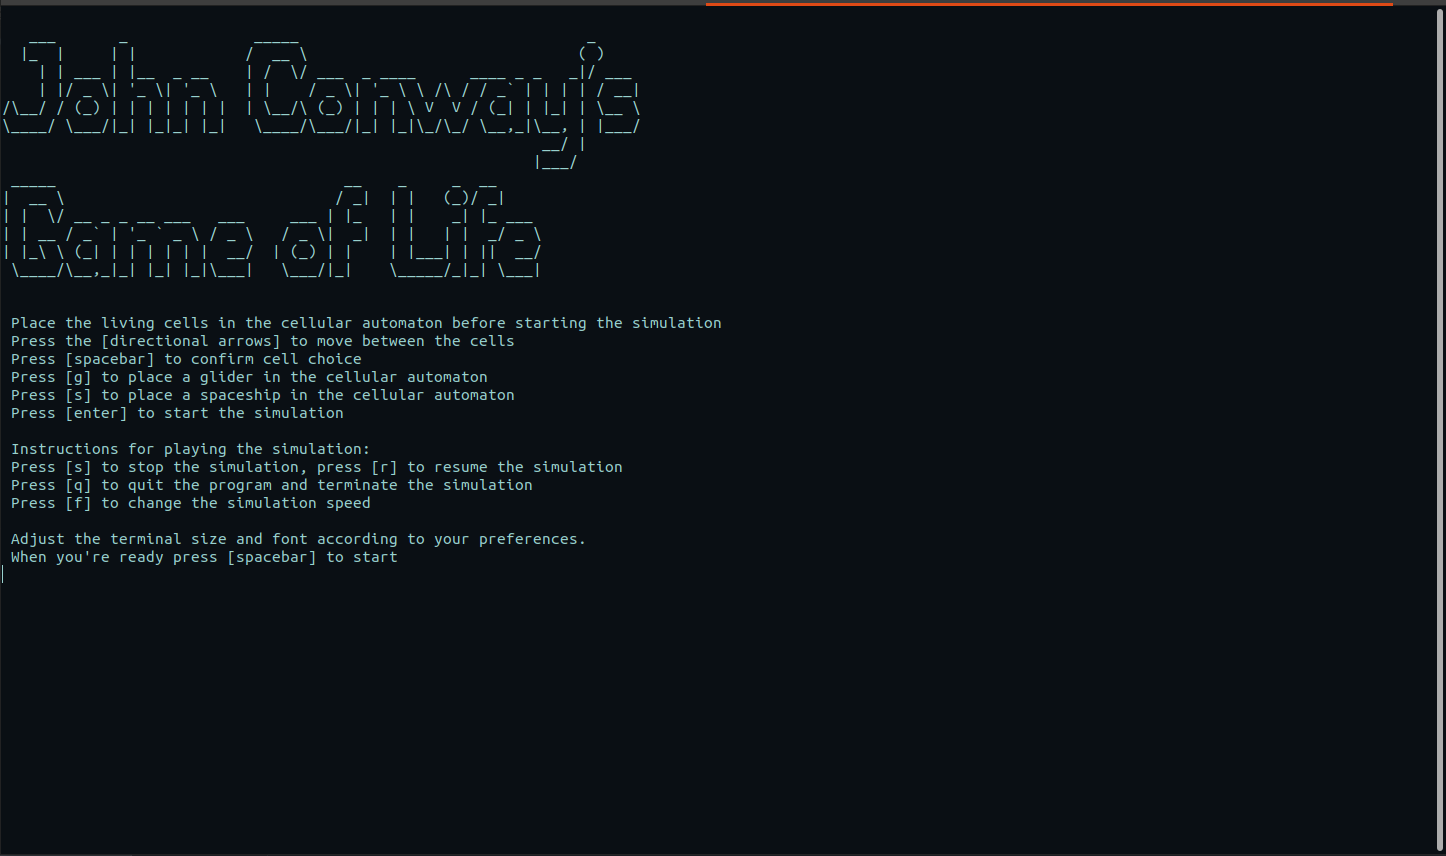
\includegraphics[width=0.75\textwidth]{images/prompt.png}
    \caption{Initial game prompt with tutorial}
    \label{fig:prompt}
\end{figure}

\begin{figure}[h]
    \centering
    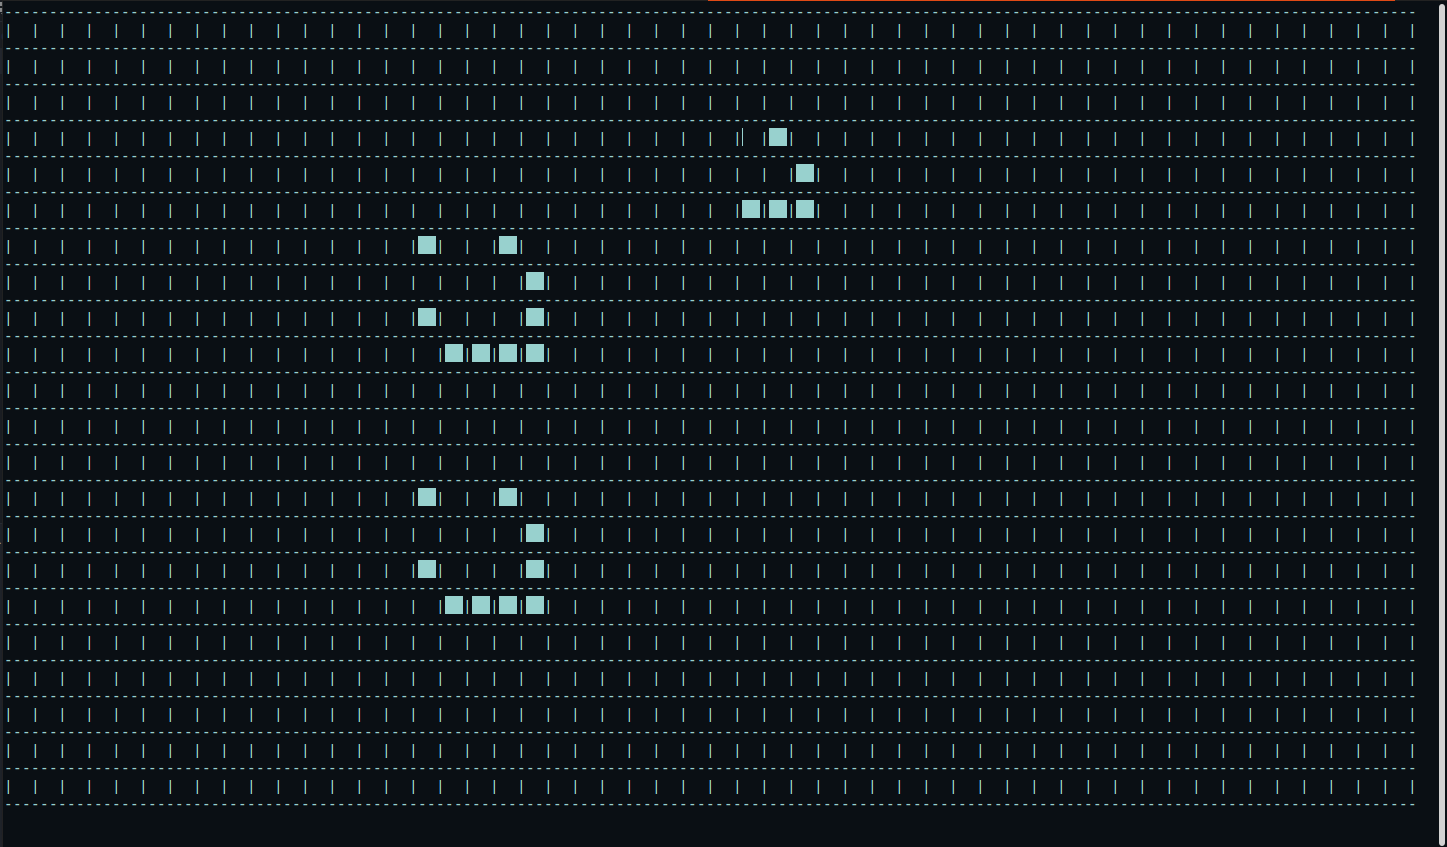
\includegraphics[width=0.75\textwidth]{images/game.png}
    \caption{Initial game setup with 2 spaceships and a glider}
    \label{fig:initialize}
\end{figure}

\begin{figure}[h!]
    \centering
    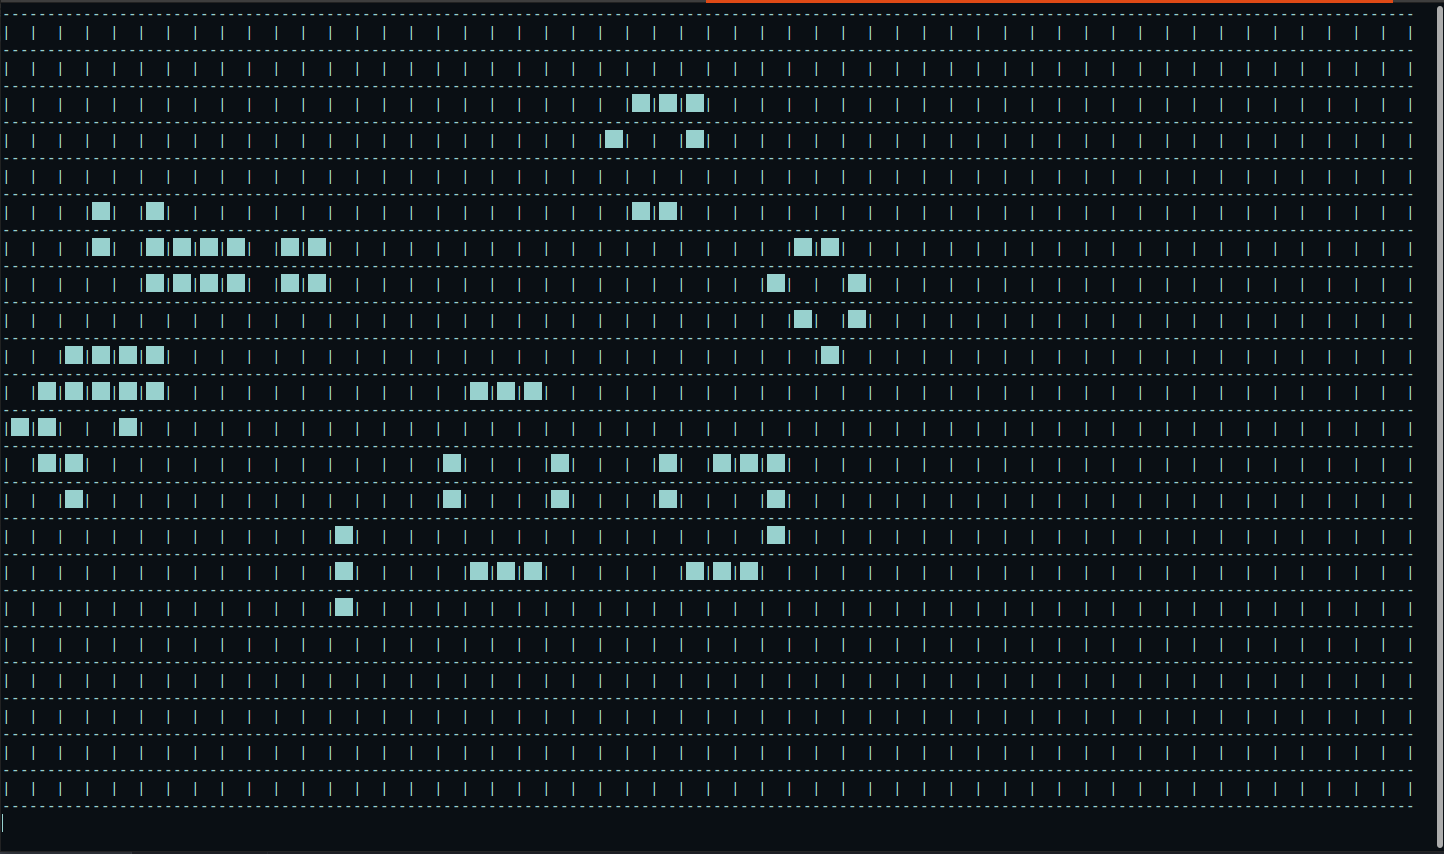
\includegraphics[width=0.75\textwidth]{images/game2.png}
    \caption{An example of a frame from another simulation}
    \label{fig:running}
\end{figure}

\subsection{Learning opportunity}

The project source code is entirely written in C++. I didn't have any prior coding experience with C++, so this project enabled me to learn and practice C++ programming.
Furthermore, I put in practice the acquired knowledge about concurrent and multi-threading programming in a real time embedded system environment, which is a very useful field to have experience with. 
I'm really interested in working in the embedded systems field, and this project showed me that I would like to pursue this career field, even though I found that it's quite difficult to approach, especially for novices. 

\subsection{Existing knowledge}

I attended the ACSO course (Computer Architectures and Operating Systems), which gave me the necessary knowledge and understanding about how operating systems work, so that made it possible to attend the AOS course and complete this project.
My prior knowledge of low level C programming and MIPS Assembly proved to be fundamental in order to comprehend the topics of the AOS course. Also reading the source code of the Miosix kernel (which was necessary in some cases in order to solve some bugs) required a deep understanding of some of the course topics covered, especially the concurrency and multi-threading part.

A quick introduction on how to use all the terminal features would have been useful though. The \verb|termios| library contains a lot of parameters, that, if used correctly, enable the programmer to create complex GUI-looking command-line utilities and programs. At first, it was not really easy to understand how it works.

\subsection{Problems encountered}
Several problems have been encountered during the development process. At first, the command line wasn't responding like it was expected. Afterwards a lot of compilation errors often popped up due to the fact that the Miosix OS doesn't implement every function in the standard libraries. 

\begin{itemize}
    \item \textbf{Command line malfunctions}\\
    The biggest problem that I faced was that new lines didn't reset the cursor position at the start of the line. 
    Basically carriage returns weren't working.
    It turns out it was neither an input or output problem, because there is no flag in the \verb|termios| data structure that could fix the problem.
    I tried setting every possible flag combination, and I eventually gave up when I realized that it was due to the raw (non canonical) mode.
    I managed to get carriage returns successfully by adding the character "\verb|\r|" at the end of every printed string, alongside the character "\verb|\n|".
    
    \item \textbf{Timeouts and timed condition variables}\\
    Timed condition variables are not currently implemented on the Miosix OS.
    I needed to apply a timeout on a function that was reading user input, but the function that reads from a file descriptor is a thread-blocking function, thus there is no way of waking up from the I/O wait after a certain time elapses.
    No alternative methods that were making use of the \verb|termios| library were working. 
    
    Also, the \verb|select| function didn't work because the corresponding library is not implemented in the Miosix OS.
    I eventually solved the problem by changing the way the main thread interacts with the reader thread, and by making the input management
    function non blocking. 
    
    \item \textbf{Slow baud rate}\\
    The standard baud rate was too slow to properly see how the cellular automaton evolved over time, because the entirety of the terminal needed to be rewritten at each displayed frame. 
    This problem was solved by increasing the baud rate to 460800, which proved to be the highest working baud rate. This way, the output is much smoother and the terminal refreshes faster.
    Even though it is still not as fast and smooth as the Linux command line executed on a pc, this is the fastest achievable speed via mini-usb serial communication.

\end{itemize}
    
    
\section{Honor Pledge}

I pledge that this work was fully and wholly completed within the criteria established for academic integrity by Politecnico di Milano
(Code of Ethics and Conduct) and represents my original production, unless otherwise cited.

I also understand that this project, if successfully graded, will fulfill part B requirement of the Advanced Operating System course
and that it will be considered valid up until the exam of September 2022. 

\begin{flushright}
Simone Giampà
\end{flushright}


\end{document}
